\let\negmedspace\undefined
\let\negthickspace\undefined
\documentclass[journal]{IEEEtran}
\usepackage[a5paper, margin=10mm, onecolumn]{geometry}
\usepackage{lmodern} % Ensure lmodern is loaded for pdflatex
\usepackage{tfrupee} % Include tfrupee package

\setlength{\headheight}{1cm} % Set the height of the header box
\setlength{\headsep}{0mm}     % Set the distance between the header box and the top of the text

\usepackage{gvv-book}
\usepackage{gvv}
\usepackage{cite}
\usepackage{amsmath,amssymb,amsfonts,amsthm}
\usepackage{algorithmic}
\usepackage{graphicx}
\usepackage{textcomp}
\usepackage{xcolor}
\usepackage{txfonts}
\usepackage{listings}
\usepackage{enumitem}
\usepackage{mathtools}
\usepackage{gensymb}
\usepackage{comment}
\usepackage[breaklinks=true]{hyperref}
\usepackage{tkz-euclide} 
\usepackage{listings}
\usepackage{gvv}                                        
\def\inputGnumericTable{}                                 
\usepackage[latin1]{inputenc}                                
\usepackage{color}                                            
\usepackage{array}                                            
\usepackage{longtable}                                       
\usepackage{calc}                                             
\usepackage{multirow}                                         
\usepackage{hhline}                                           
\usepackage{ifthen}                                           
\usepackage{lscape}
\begin{document}

\bibliographystyle{IEEEtran}
\vspace{3cm}

\title{9-9.2-37}
\author{EE24BTECH11020 - Ellanti Rohith}
% \maketitle
% \newpage
% \bigskip
{\let\newpage\relax\maketitle}
Question:\\
Draw the rough rough sketch of region $\myvec{x&y}$: $y^2<6ax$ and $x^2+y^2<16a^2$ 
\begin{table}[h!]    
  \centering
  \begin{tabular}[12pt]{ |c| c|}
    \hline
    \textbf{Variable} & \textbf{Description}\\ 
    \hline
	$\vec{e}$ & Eccentricity of conic\\
	\hline
	$\vec{F}$ & Focus of conic\\
	\hline
	$\vec{I}$ & Identity matrix\\
	\hline
	$\vec{n}^{\top}\vec{x}=c$ & Equation of directrix\\
	\hline
	$\vec{n}$ & Slope of normal to directrix\\
	\hline
	$f$ & $\norm{\vec{n}}^2\norm{\vec{F}}^2-c^2e^2$\\
	\hline
	$\vec{V}$ & A symmetric matrix given by eigenvalue decomposition\\
	\hline
	$\vec{u}$ & Vertex of conic with same directrix\\
	\hline
\end{tabular}

  \caption{Variables Used}
  \label{tab1-9.2.1}
\end{table}\\
\solution
The general equation of a parabola with directrix $\vec{n}^{\top}\vec{x}=c$ is given by,
\begin{align}
	g\brak{\vec{x}}=\vec{x}^{\top}\vec{V}\vec{x}+2\vec{u}^{\top}\vec{x}+f=0\\
	\vec{V}=\norm{\vec{n}}^2\vec{I}-e^2\vec{n}\vec{n}^{\top}\\
	\vec{u}=ce^2\vec{n}-\norm{\vec{n}}^2\vec{F}\\
	f=\norm{\vec{n}}^2\norm{\vec{F}}^2-c^2e^2
\end{align}
for the parabola $y^2=6ax$, equation of directrix is, $\myvec{2&0}\vec{x}=-3a$
\begin{align}
	\vec{V}&=\myvec{0&0\\0&1}\\
	\vec{u}&=\myvec{-3a\\0}\\
	f&=0
\end{align}
The given circle can be expressed as conics with parameters
\begin{align}
	\vec{V}&=\myvec{4a&0\\0&4a}\\
	\vec{u}&=0\\
	f&=-16a^2
\end{align}

The intersection of two conics with parameters $\vec{V}_i,\vec{u}_i,f_i, i=1,2$ is defined as,
\begin{align}
	\vec{x}^{\top}\brak{\vec{V}_1-\vec{V}_2}\vec{x}+2\brak{\vec{u}_1-\vec{u_2}}^{\top}\vec{x}+\brak{f_1-f_2}=0
\end{align} 
On solving we get the points of intersection to be $2a\myvec{1\\ \sqrt{3}},2a\myvec{1\\-\sqrt{3}}$

\begin{figure}[h!]
   \centering
   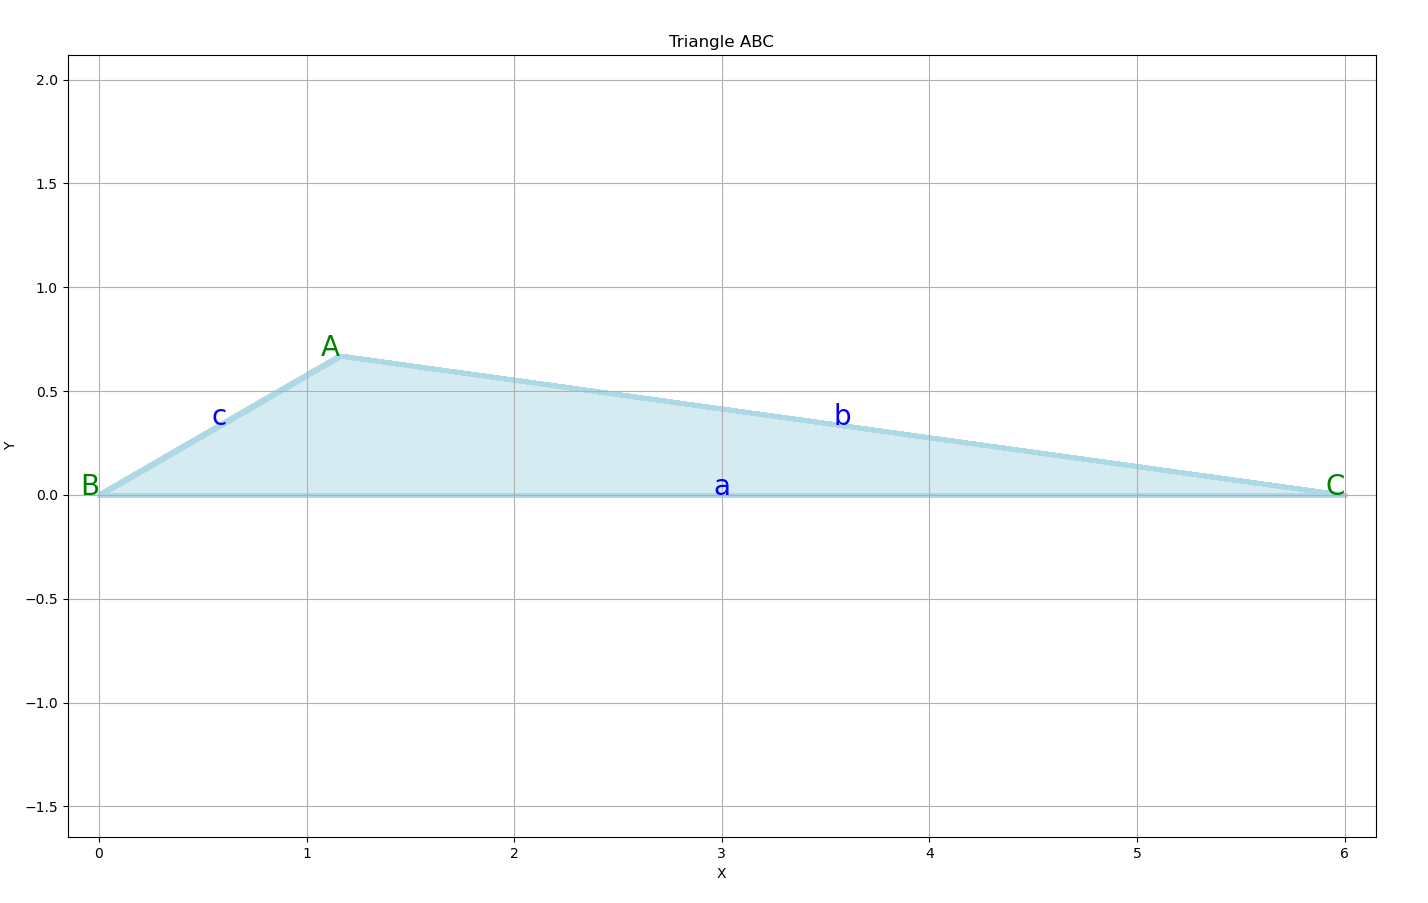
\includegraphics[width = 1\linewidth]{figs/fig.png}
   \caption{Sketch of given region}
   \label{stemplot}
\end{figure}
\end{document}
